\documentclass[11pt,a4paper]{article}


\usepackage[utf8]{inputenc}
\usepackage[T1]{fontenc}
\usepackage{lmodern}
\usepackage{microtype}
\usepackage[margin=2.2cm]{geometry}
\usepackage{graphicx}
\usepackage{xcolor}
\usepackage{listings}
\usepackage{booktabs}
\usepackage{enumitem}
\usepackage{hyperref}
\usepackage{titlesec}
\usepackage{fancyhdr}

\hypersetup{
    colorlinks=true,
    linkcolor=blue,
    urlcolor=blue,
    citecolor=blue
}

\titleformat{\section}{\Large\bfseries\color{black!85}}{\thesection}{1em}{}
\titleformat{\subsection}{\large\bfseries\color{black!75}}{\thesubsection}{1em}{}

\pagestyle{fancy}
\fancyhf{}
\fancyhead[L]{DevOps Project -- Deploying an Open-Source LLM}
\fancyhead[R]{\thepage}
\renewcommand{\headrulewidth}{0.4pt}
\setlength{\headheight}{14pt}

\definecolor{codebg}{RGB}{245,245,245}
\lstset{
    backgroundcolor=\color{codebg},
    basicstyle=\ttfamily\small,
    breaklines=true,
    frame=single,
    framesep=4pt,
    columns=fullflexible,
    keywordstyle=\color{blue!70!black},
    commentstyle=\color{gray}
}

\title{\vspace{-1.5cm}\textbf{Déploiement d'un LLM Open-Source \\ avec Docker Compose et Kubernetes}\\[0.3cm]
\large Rapport de projet DevOps}
\author{}
\date{}

\begin{document}

\maketitle
\thispagestyle{fancy}
\vspace{-1.2cm}

\section*{Introduction}

Ce projet a pour objectif de déployer une application d'intelligence artificielle conteneurisée --- un serveur de modèles de langage (\textbf{Ollama}) couplé à une interface web de conversation (\textbf{Open WebUI}) --- d'abord localement avec Docker Compose, puis sur un cluster Kubernetes (Minikube), en appliquant les bonnes pratiques d'orchestration de conteneurs. Ce rapport présente l'architecture retenue, explique le rôle de chaque ressource Kubernetes créée, détaille le mécanisme de communication entre les services, justifie l'usage du stockage persistant et des sondes de santé, et conclut par une comparaison entre Docker Compose et Kubernetes.

\section{Architecture de l'application}

L'application repose sur deux services conteneurisés qui communiquent en réseau interne :

\begin{itemize}[nosep]
    \item \textbf{Ollama} : héberge et exécute les modèles de langage (\texttt{llama3.2:3b} et \texttt{mistral:7b} dans ce projet). Il expose une API HTTP sur le port \texttt{11434}.
    \item \textbf{Open WebUI} : interface web de type chat (similaire à ChatGPT), qui interroge l'API d'Ollama pour générer des réponses. Elle expose son interface sur le port \texttt{8080}.
\end{itemize}

Cette architecture a d'abord été validée avec Docker Compose (fichier \texttt{docker-compose.yaml}), puis reproduite intégralement avec des manifestes Kubernetes.

\section{Déploiement Kubernetes : rôle de chaque ressource}

Le déploiement Kubernetes est composé de neuf manifestes YAML, appliqués dans le namespace dédié \texttt{llm-devops}. Chaque ressource a une responsabilité précise.

\subsection{Namespace}

Le \texttt{Namespace llm-devops} isole l'ensemble des ressources du projet du reste du cluster. Il agit comme un espace de nommage logique : toutes les autres ressources (Deployments, Services, PVC, ConfigMap) y sont rattachées, ce qui simplifie la gestion, le nettoyage et évite les collisions de noms avec d'autres applications.

\subsection{ConfigMap}

Le \texttt{ConfigMap llm-config} centralise la configuration de l'application (URL interne d'Ollama, paramètres \texttt{OLLAMA\_KEEP\_ALIVE}, désactivation du téléchargement automatique des modèles d'embedding RAG, etc.). Les deux \texttt{Deployments} l'importent via \texttt{envFrom}. Cette approche remplace les variables d'environnement codées en dur : une modification de configuration ne nécessite pas de reconstruire les images ni de modifier les Deployments.

\subsection{PersistentVolumeClaim (PVC)}

Deux PVC ont été créés :
\begin{itemize}[nosep]
    \item \texttt{ollama-pvc} (15 Gi) : stocke les poids des modèles téléchargés (\texttt{/root/.ollama}).
    \item \texttt{webui-pvc} (2 Gi) : stocke la base de données d'Open WebUI (comptes utilisateurs, historique des conversations).
\end{itemize}

Voir la section~\ref{sec:pvc} pour la justification détaillée de leur nécessité.

\subsection{Deployments}

Les \texttt{Deployments ollama} et \texttt{open-webui} définissent chacun un pod avec : l'image du conteneur, les points de montage vers les PVC, les variables issues du ConfigMap, les requêtes et limites de ressources CPU/mémoire, ainsi que les trois sondes de santé (voir section~\ref{sec:probes}). Un Deployment garantit qu'un pod correspondant à cette spécification tourne en permanence : en cas de crash, Kubernetes le redémarre automatiquement, et en cas de mise à jour de configuration (\texttt{kubectl apply}), il orchestre un remplacement progressif du pod (rolling update) sans interruption de service.

\subsection{Services}

Deux \texttt{Services} de type \texttt{ClusterIP} (\texttt{ollama} et \texttt{open-webui}) exposent chaque Deployment via une adresse réseau stable. Leur rôle est détaillé en section~\ref{sec:communication}.

\subsection{Ingress}

L'\texttt{Ingress open-webui-ingress} définit une route HTTP externe (\texttt{llm.local} $\rightarrow$ \texttt{open-webui:8080}) via un contrôleur \texttt{nginx}. Sur l'environnement de test (Minikube avec driver Docker sous Windows), l'accès direct à l'adresse du nœud n'étant pas routable depuis l'hôte sans configuration réseau supplémentaire (\texttt{minikube tunnel}), l'accès effectif pour les tests a été réalisé via \texttt{kubectl port-forward}, solution de repli explicitement acceptée par l'énoncé du projet. Le manifeste Ingress reste néanmoins fonctionnel et démontre la connaissance de ce mécanisme d'exposition.

\section{Communication entre les services}
\label{sec:communication}

Kubernetes attribue à chaque pod une adresse IP interne, mais celle-ci change à chaque redémarrage : elle ne peut donc pas être utilisée comme référence stable. Les \textbf{Services} résolvent ce problème en fournissant une adresse virtuelle stable (ClusterIP) associée à un nom DNS interne au cluster, résolu automatiquement par CoreDNS.

Concrètement, le Service \texttt{ollama} expose le pod Ollama sous le nom \texttt{ollama} (résolu en \texttt{ollama.\allowbreak llm-devops.\allowbreak svc.\allowbreak cluster.\allowbreak local}, ou simplement \texttt{ollama} au sein du même namespace). C'est exactement l'URL déclarée dans le ConfigMap :

\begin{lstlisting}
OLLAMA_BASE_URL: "http://ollama:11434"
\end{lstlisting}

Le pod Open WebUI utilise cette variable pour contacter l'API d'Ollama, quelle que soit l'IP réelle du pod Ollama à un instant donné. Le Service fait office de load-balancer interne et de point d'indirection stable : si le pod Ollama est recréé (crash, mise à jour), son IP change mais le Service et son nom DNS restent identiques, garantissant la continuité de la communication. Ce mécanisme remplace le réseau bridge nommé (\texttt{networks: llm}) utilisé dans Docker Compose, où la résolution de noms de conteneurs jouait un rôle équivalent mais plus rudimentaire.

\section{Pourquoi les PersistentVolumeClaims sont nécessaires}
\label{sec:pvc}

Par défaut, le système de fichiers d'un conteneur est \textbf{éphémère} : toute donnée écrite est perdue dès que le conteneur est recréé (redémarrage suite à un crash, mise à jour du Deployment, ou reprogrammation sur un autre nœud). Or deux types de données doivent impérativement survivre à ces événements :

\begin{itemize}[nosep]
    \item les poids des modèles LLM téléchargés dans Ollama (plusieurs gigaoctets, coûteux à retélécharger) ;
    \item la base de données d'Open WebUI (comptes utilisateurs, historique des conversations).
\end{itemize}

Un \texttt{PersistentVolumeClaim} découple le cycle de vie du stockage de celui du pod : les données sont écrites sur un volume physique (ici provisionné automatiquement par le \texttt{storage-provisioner} de Minikube) qui persiste indépendamment du pod qui l'utilise. Ce comportement a été vérifié concrètement au cours du projet : lors de l'ajustement des limites de ressources du Deployment Ollama (voir section~\ref{sec:incidents}), le pod a été recréé plusieurs fois, et les modèles \texttt{llama3.2:3b} et \texttt{mistral:7b} sont restés disponibles sans nouveau téléchargement, confirmant le bon fonctionnement du PVC.

\section{Rôle des sondes de santé (probes)}
\label{sec:probes}

Chaque conteneur des Deployments est équipé de trois sondes complémentaires, interrogeant un point de terminaison HTTP (\texttt{/api/version} pour Ollama, \texttt{/health} pour Open WebUI) :

\begin{itemize}
    \item \textbf{Startup Probe} : vérifie que l'application a fini son démarrage avant que les autres sondes ne soient prises en compte. Elle tolère un délai de démarrage long (jusqu'à 150 secondes ici) sans déclencher de redémarrage prématuré du conteneur --- utile car le serveur Ollama ou Open WebUI peut mettre du temps à devenir disponible au premier lancement.
    \item \textbf{Readiness Probe} : détermine si le pod est prêt à recevoir du trafic. Si elle échoue, le pod est retiré des endpoints du Service (le trafic n'y est plus routé) sans que le conteneur soit redémarré --- utile lors d'une surcharge temporaire.
    \item \textbf{Liveness Probe} : détermine si le conteneur est toujours fonctionnel. Si elle échoue de façon répétée, Kubernetes redémarre le conteneur, permettant de récupérer automatiquement d'un blocage applicatif (deadlock, fuite mémoire).
    \end{itemize}

Ces sondes ne sont pas restées théoriques dans ce projet : le pod Open WebUI a initialement échoué sa \texttt{startupProbe} car l'application tentait de télécharger un modèle d'embedding HuggingFace (\texttt{sentence-transformers/all-MiniLM-L6-v2}) au démarrage, opération plus longue que le délai initialement prévu. La correction a consisté à désactiver ce téléchargement non nécessaire pour ce projet (\texttt{RAG\_EMBEDDING\_MODEL\_AUTO\_UPDATE=false}) plutôt qu'à simplement allonger le délai, ce qui illustre l'utilité des probes pour détecter un comportement de démarrage anormal.

\section{Gestion des ressources : retour d'expérience}
\label{sec:incidents}

La définition des \texttt{requests} et \texttt{limits} CPU/mémoire a nécessité plusieurs itérations, ce qui a permis de mieux comprendre leur rôle :

\begin{itemize}
    \item \textbf{OOMKilled (mémoire insuffisante)} : la limite mémoire initiale d'Open WebUI (512 Mi) était trop basse et provoquait un \texttt{CrashLoopBackOff} (\texttt{OOMKilled}, code de sortie 137). Portée à 2 Gi, le pod a démarré normalement.
    \item \textbf{Limite CPU trop restrictive} : le modèle \texttt{mistral:7b} (7 milliards de paramètres, inférence CPU) ne produisait aucune réponse après plus de dix minutes avec une limite de 2 vCPU. Le noeud disposant de 8 coeurs logiques, la limite a été relevée à 6 vCPU, ramenant le temps de première réponse à moins de 70 secondes (chargement du modèle inclus).
\end{itemize}

Ces incidents illustrent concrètement pourquoi les \texttt{requests} (ressources garanties, utilisées pour l'ordonnancement) et les \texttt{limits} (plafond dur, au-delà duquel le conteneur est limité ou tué) doivent être dimensionnées en fonction de la charge réelle de l'application, et non de valeurs arbitraires.

\section{Différences entre Docker Compose et Kubernetes}

\begin{table}[h]
\centering
\small
\begin{tabular}{@{}p{4.2cm}p{5.3cm}p{5.3cm}@{}}
\toprule
\textbf{Aspect} & \textbf{Docker Compose} & \textbf{Kubernetes} \\
\midrule
Portée & Un seul hôte Docker & Cluster de plusieurs noeuds \\
Déclaration & Un seul fichier YAML & Plusieurs manifestes granulaires (Namespace, Deployment, Service, etc.) \\
Résilience & Redémarrage simple (\texttt{restart: unless-stopped}) & Auto-guérison avancée via Deployments, ReplicaSets et probes \\
Mise à l'échelle & Manuelle, limitée (\texttt{--scale}) & Native, avec support d'auto-scaling (HPA) \\
Réseau & Réseau bridge nommé, résolution par nom de conteneur & Services + CoreDNS, load-balancing interne \\
Stockage & Volumes Docker nommés & PersistentVolumeClaims avec provisionnement dynamique \\
Santé & Un seul \texttt{healthcheck} par service & Trois sondes distinctes (startup/readiness/liveness) aux rôles différenciés \\
Cas d'usage & Développement local, prototypage & Production, haute disponibilité, orchestration à grande échelle \\
\bottomrule
\end{tabular}
\caption{Comparaison synthétique entre Docker Compose et Kubernetes}
\end{table}

En résumé, Docker Compose reste pertinent pour un développement local rapide sur une seule machine, tandis que Kubernetes apporte les mécanismes nécessaires à une exploitation en production : résilience automatisée, découplage explicite des responsabilités, gestion fine des ressources et capacité de montée en charge.

\section{Validation du déploiement}

Le déploiement a été validé selon les critères suivants, conformément aux exigences du projet :

\begin{itemize}[nosep]
    \item les deux pods sont à l'état \texttt{Running} (voir figure~\ref{fig:pods});
    \item aucun pod n'est en \texttt{CrashLoopBackOff} ni en \texttt{Pending} ;
    \item Open WebUI communique correctement avec Ollama via le Service interne ;
    \item la page d'accueil d'Open WebUI est accessible via le déploiement Kubernetes (figure~\ref{fig:webui}) ;
    \item les modèles \texttt{llama3.2:3b} et \texttt{mistral:7b} sont disponibles et répondent aux invites (figures~\ref{fig:llama} et~\ref{fig:mistral}).
\end{itemize}

\begin{figure}[h]
    \centering
    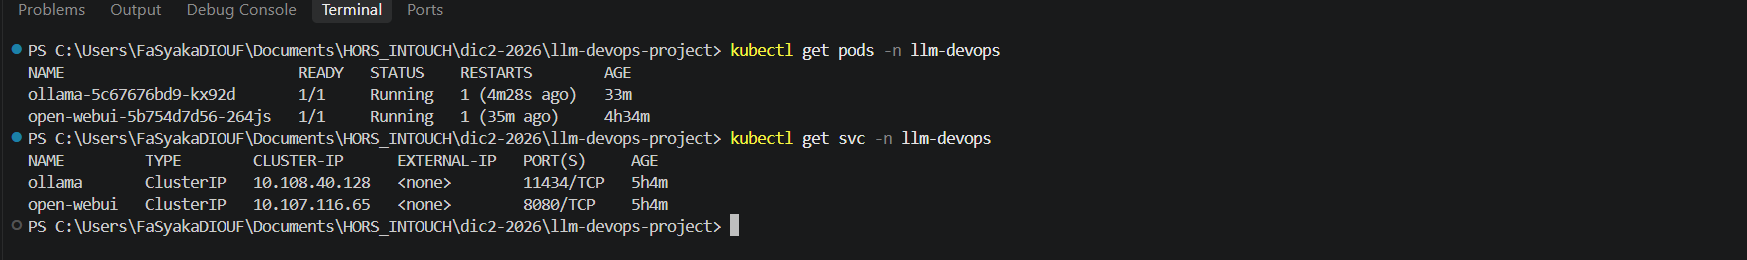
\includegraphics[width=0.85\textwidth]{../screenshots/pods_services_running.png}
    \caption{Pods et Services Kubernetes en fonctionnement (\texttt{kubectl get pods} / \texttt{kubectl get svc})}
    \label{fig:pods}
\end{figure}

\begin{figure}[h]
    \centering
    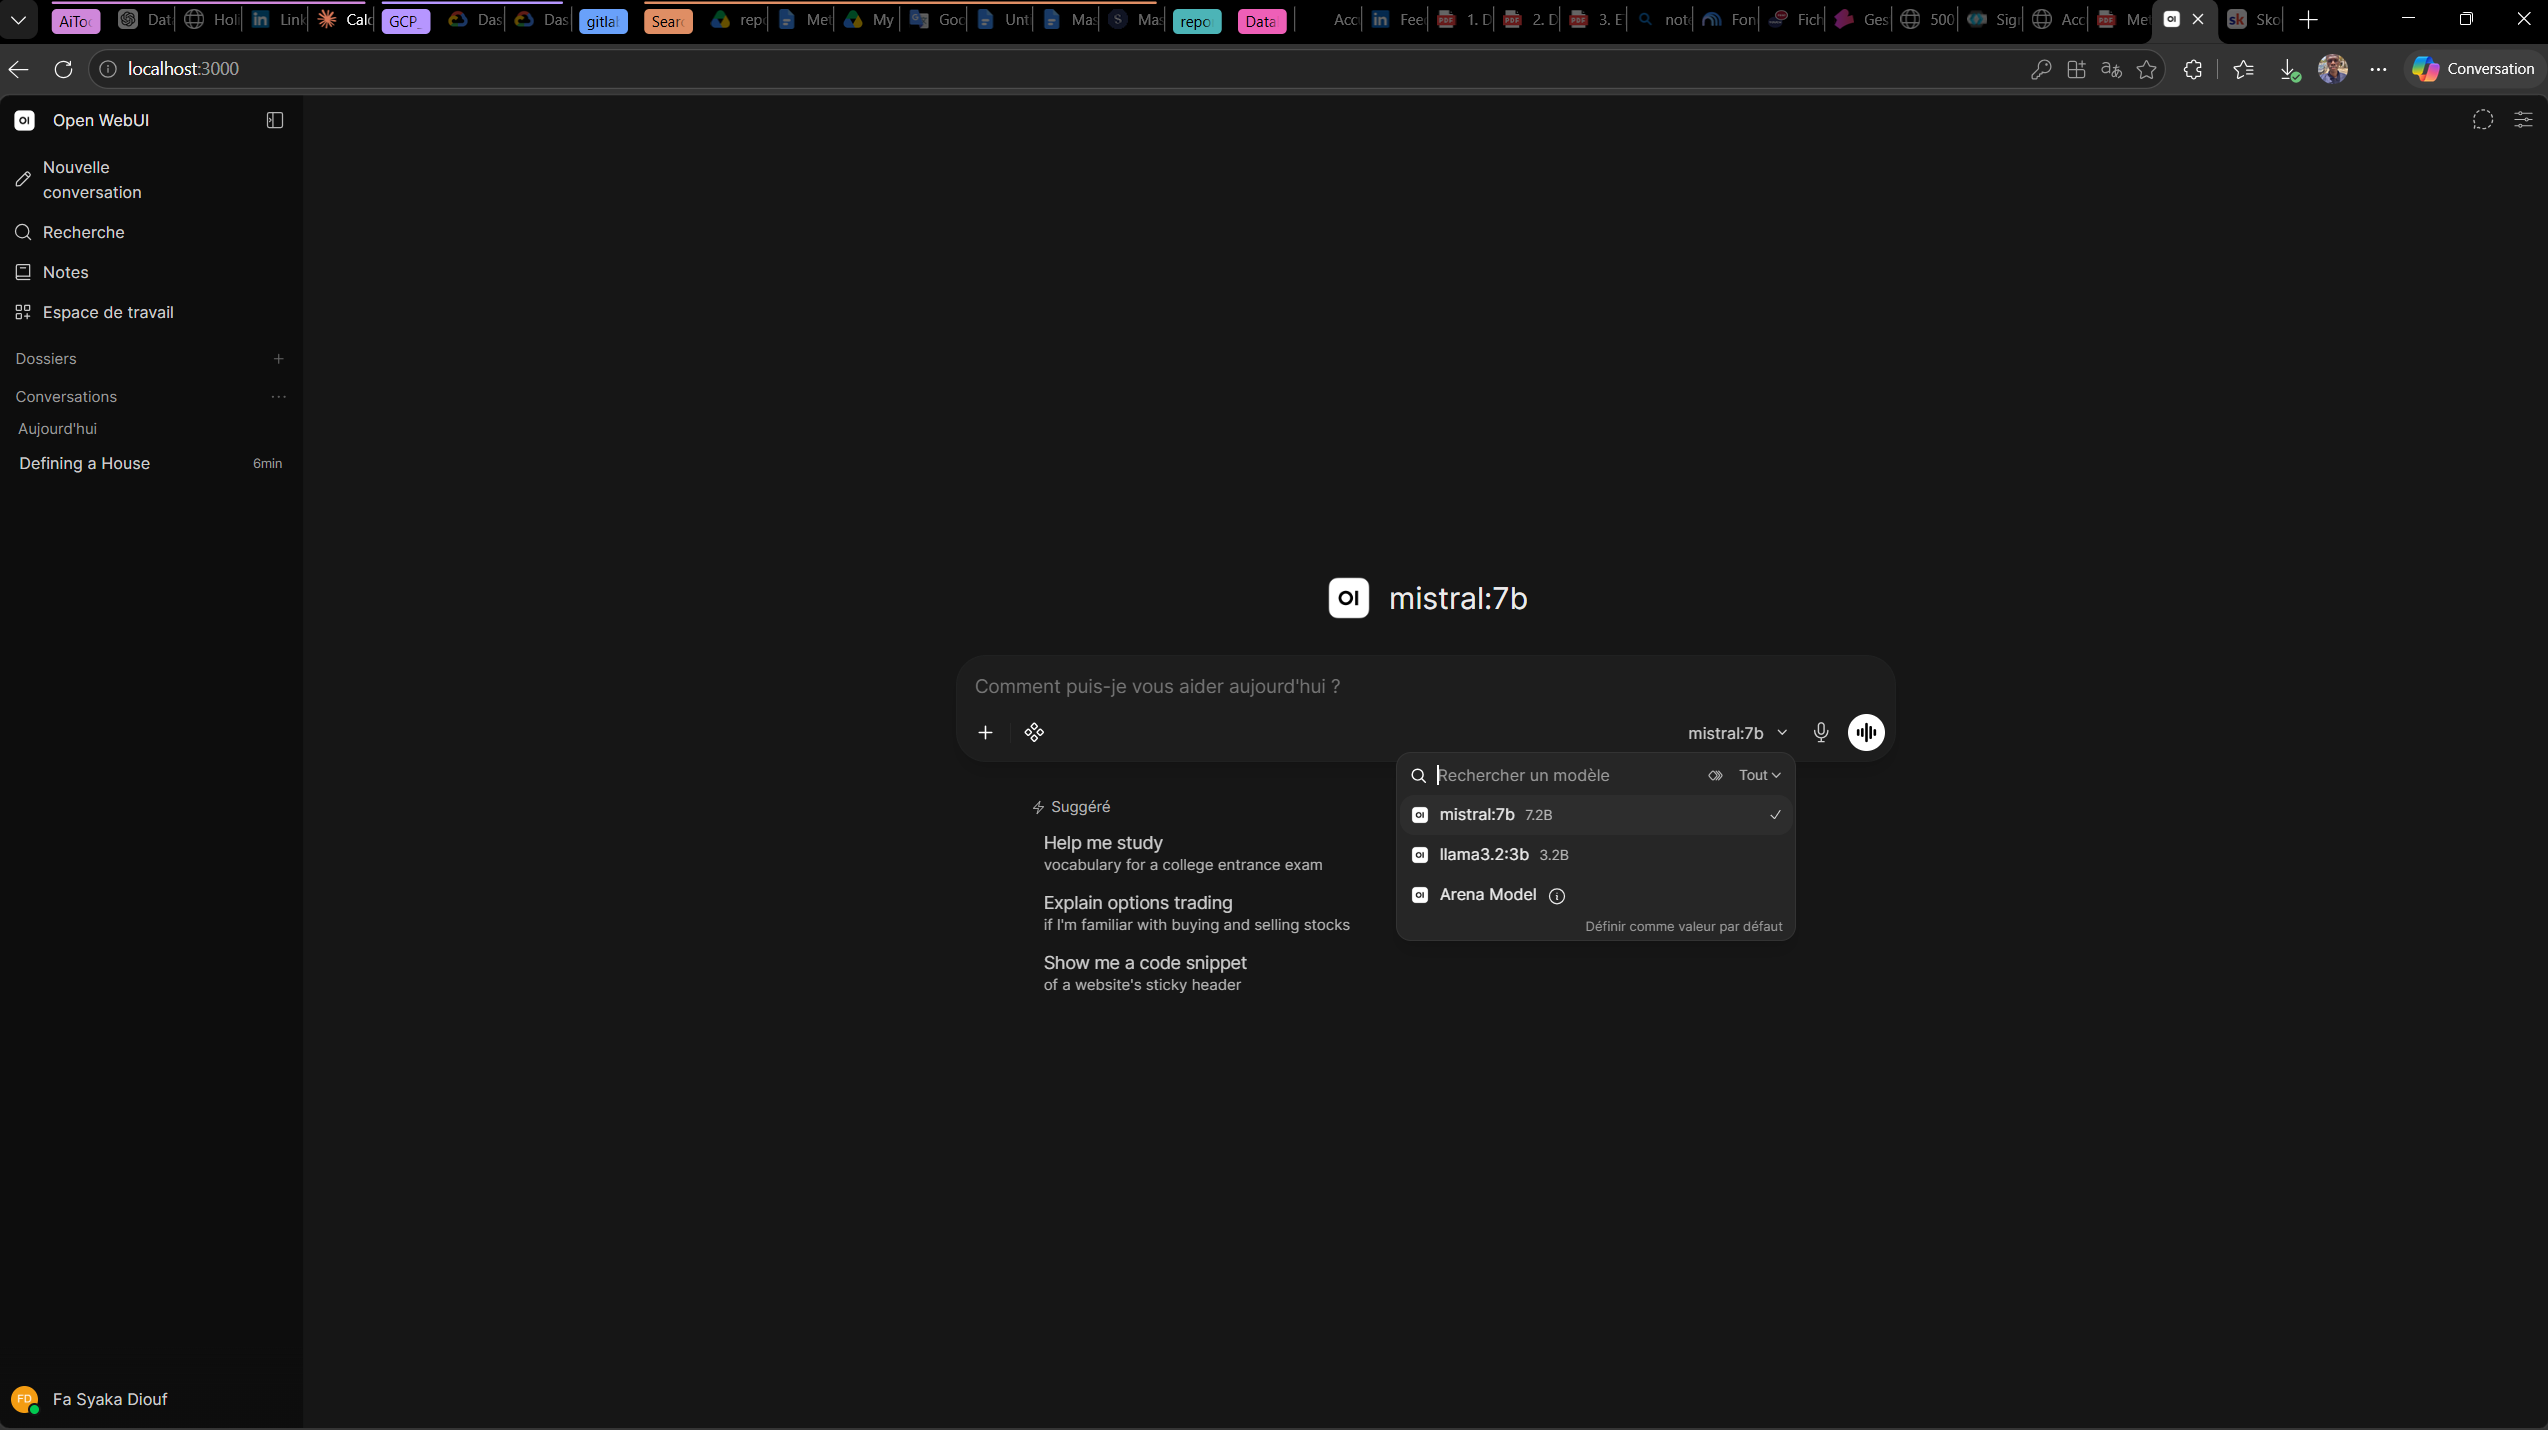
\includegraphics[width=0.85\textwidth]{../screenshots/open_webui_kubernetes.png}
    \caption{Page d'accueil d'Open WebUI, servie par le déploiement Kubernetes}
    \label{fig:webui}
\end{figure}

\begin{figure}[h]
    \centering
    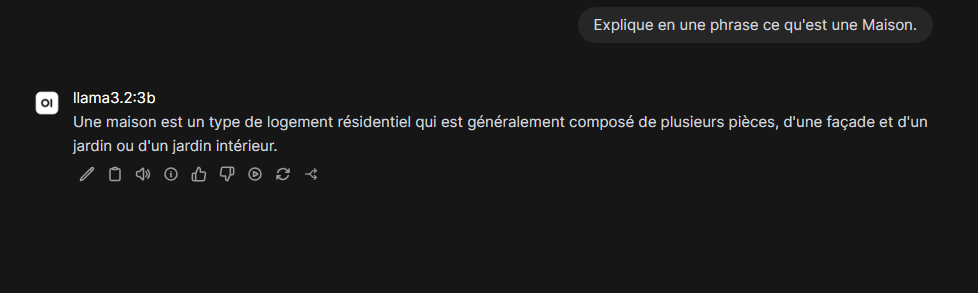
\includegraphics[width=0.85\textwidth]{../screenshots/prompt-llama-kubernets.png}
    \caption{Réponse générée par le modèle llama3.2:3b}
    \label{fig:llama}
\end{figure}

\begin{figure}[h]
    \centering
    
\includegraphics[width=0.85\textwidth]{../screenshots/prompt-mistral-kubernet.png}
    \caption{Réponse générée par le modèle mistral:7b}
    \label{fig:mistral}
\end{figure}

\section*{Conclusion}

Ce projet a permis de mettre en pratique l'ensemble du cycle de conteneurisation d'une application d'IA, depuis un déploiement local avec Docker Compose jusqu'à une orchestration Kubernetes conforme aux bonnes pratiques de production (isolation par namespace, configuration externalisée, stockage persistant, gestion explicite des ressources, sondes de santé multi-niveaux). Les difficultés rencontrées en conditions réelles --- limite mémoire trop basse, quota CPU insuffisant pour l'inférence d'un modèle de 7 milliards de paramètres, téléchargement bloquant au démarrage --- ont constitué des cas d'étude concrets pour comprendre le rôle exact de chaque mécanisme Kubernetes plutôt qu'une simple application théorique du cours.

\end{document}